\documentclass{acmsiggraph}                     % final
%\documentclass[annualconference]{acmsiggraph}  % final (annual conference)
%\documentclass[review]{acmsiggraph}            % review
%\documentclass[widereview]{acmsiggraph}        % wide-spaced review
%\documentclass[preprint]{acmsiggraph}          % preprint

%% Uncomment one of the five lines above depending on where your paper is
%% in the conference process. ``review'' and ``widereview'' are for review
%% submission, ``preprint'' is for pre-publication, and ``final'' is for
%% the version to be printed. The ``final'' variant will accept the 
%% ``annualconference'' parameter, which changes the height of the space
%% left clear for the ACM copyright information.

%% The 'helvet' and 'times' packages define the typefaces used for
%% serif and sans serif type in this document. Computer Modern Roman 
%% is used for mathematics typesetting. The scale factor is set to .92
%% to bring the sans-serif type in line with the serif type.

\usepackage[scaled=.92]{helvet}
\usepackage{times}

%% The 'graphicx' package allows for the inclusion of EPS figures.

\usepackage{graphicx}

%% use this for zero \parindent and non-zero \parskip, intelligently.

\usepackage{parskip}

%% Optional: the 'caption' package provides a nicer-looking replacement
%% for the standard caption environment. With 'labelfont=bf,'textfont=it',
%% caption labels are bold and caption text is italic.

\usepackage[labelfont=bf,textfont=it]{caption}

%% If you are submitting a paper to the annual conference, please replace 
%% the value ``0'' below with the numeric value of your OnlineID. 
%% If you are not submitting this paper to the annual conference, 
%% you may safely leave it at ``0'' -- it will not be included in the output.

\onlineid{0}

%% Paper title.

\title{News Knitter}

%% Author and Affiliation (single author).

%%\author{Roy G. Biv\thanks{e-mail: roy.g.biv@aol.com}\\Allied Widgets Research}

%% Author and Affiliation (multiple authors).

\author{Ebru Kurbak\thanks{e-mail:ebru.kurbak@ufg.ac.at}\\ University of Art and Industrial Design Linz %
\and Mahir M. Yavuz\thanks{e-mail:mahir.yavuz@ufg.ac.at}\\University of Art and Industrial Design Linz}

%% Keywords that describe your work.

\keywords{radiosity, global illumination, constant time}

%%%%%% START OF THE PAPER %%%%%%

\begin{document}

\teaser{
  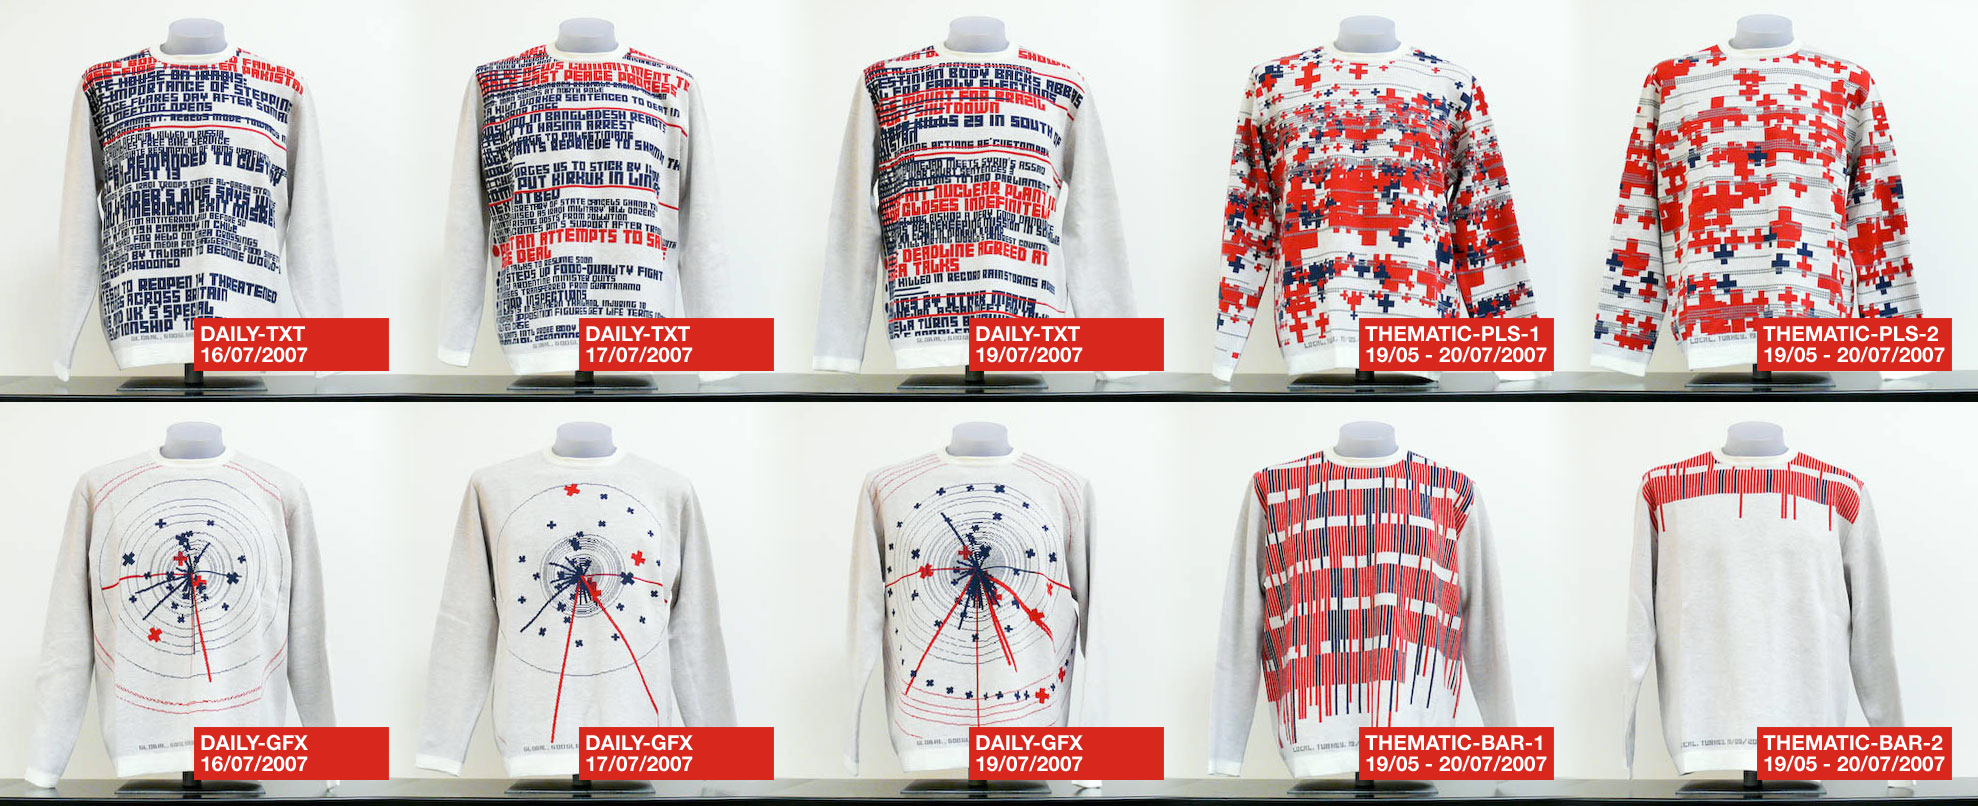
\includegraphics[width=6in]{00-nk-sweaters-full.png}
  \caption{News Knitter Sweaters}
}

%% The ``\maketitle'' command must be the first command after the
%% ``\begin{document}'' command. It prepares and prints the title block.

\maketitle

%% Abstract section.

%% \begin{abstract}

%% Duis autem vel eum iriure dolor in hendrerit in vulputate velit esse
%% molestie consequat, vel illum dolore eu feugiat nulla facilisis at 
%% vero eros et accumsan et iusto odio dignissim qui blandit praesent
%% luptatum zzril delenit augue duis dolore te feugait nulla
%% facilisi. Lorem ipsum dolor sit amet, consectetuer adipiscing elit,
%% sed diam nonummy nibh euismod tincidunt ut laoreet dolore magna
%% aliquam erat volutpat.

%% Citations can be done this way~\cite{Jobs95} or this more concise 
%% way~\shortcite{Jobs95}, depending upon the application.

%% Ut wisi enim ad minim veniam, quis nostrud exerci tation ullamcorper
%% suscipit lobortis nisl ut aliquip ex ea commodo consequat. Duis autem
%% vel eum iriure dolor in hendrerit~\cite{Pellacini:2005:LAH}
%% in vulputate velit esse molestie~\cite{notes2002} 
%% consequat, vel illum dolore eu feugiat nulla facilisis at vero eros et
%% accumsan et iusto odio dignissim qui blandit praesent luptatum zzril
%% delenit augue duis dolore te feugait nulla facilisi.~\cite{Park:2006:DSI}

%% \end{abstract}

%% ACM Computing Review (CR) categories. 
%% See <http://www.acm.org/class/1998/> for details.
%% The ``\CRcat'' command takes four arguments.

%% \begin{CRcatlist}
%%   \CRcat{K.6.1}{Management of Computing and Information Systems}%
%% {Project and People Management}{Life Cycle};
%%   \CRcat{K.7.m}{The Computing Profession}{Miscellaneous}{Ethics}
%% \end{CRcatlist}

%% The ``\keywordlist'' command prints out the keywords.
%% \keywordlist

%% \begin{abstract}

%% The ``\copyrightspace'' command must be the first command after the 
%% start of the first section of the body of your paper. It ensures the
%% copyright space is left at the bottom of the first column on the first
%% page of your paper.

%% \copyrightspace

%% \end{abstract}

\section{Patterns}

The first collection of News Knitter consists of ten unique sweaters. Patterns of these sweaters are generated by using two different live data sources and analyzing-filtering algorithms.



\subsection{Daily Patterns}

One set of patterns is generated with online global news of a particular day. Live global news items which were broadcasted within 24 hours are analyzed and filtered according to their time of publishing and their popularity. The filtered data is then visualized in two different graphic styles.

\subsubsection{DAILY-TXT}
Headlines of news items are arranged according to their time of publishing. The point size of the headline, the radius of the bullets next to the headlines and the length of the horizontal lines indicate the popularity of a particular item. All graphical elements of a news item are normally in dark blue. If a news item has been published in over 700 different sources, the color of its elements turns into red.

\subsubsection{DAILY-GFX}
Every news item is represented by a circle, a line and a plus sign. The radius of the circles, the length of the lines and the size of the plus signs indicate the popularity news items. All graphical elements of a news item are normally in dark blue. If a news item has been published in over 700 different sources, the color of its elements turns into red.

\subsection{Thematic Patterns}
Second set of patterns is generated with local Turkish news of a period based on particular themes. Each theme is expressed through two complementary keywords. Two main themes were designated for the first collection of News Knitter expressed with the keywords military-education and Asia-Europe. Live local Turkish news items broadcasted within 3 months are analyzed and filtered according to their contextual association with the predefined pairs of keywords. The frequency of appearance of the complementary keywords in news items is compared. The filtered data is then visualized in two different graphic styles.


\subsubsection{THEMATIC-BAR}
Each bar represents a news item that is associated with one of the complementary keywords arranged chronologically from upper left to lower right. Each of the two colors represents a keyword. For the first theme, red represents Europe whereas blue represents Asia and for the second theme, red represents military whereas blue represents education. The length of the bars depends on the frequency of the repetition of a keyword in a single news item.

\subsubsection{THEMATIC-PLS}
Each plus sign and gray dot represents a news item arranged chronologically from upper left to lower right. The gray dots represent the irrelevant news items that are not associated with any keyword. Each of the other two colors represents a keyword. For the first theme, red represents Europe whereas blue represents Asia and for the second theme, red represents military whereas blue represents education. The size of the plus signs depends on the frequency of the repetition of a keyword in a single news item.


\bibliographystyle{acmsiggraph}
\nocite{*}
\bibliography{template}
\end{document}
